% EpiScope - CSE 4345 CEP technical report (IEEE conference format).
% Build: make report   (numbers come from docs/report/generated/*.tex, written by orchestration/collect_results.py)
\documentclass[conference]{IEEEtran}
\IEEEoverridecommandlockouts
\usepackage[T1]{fontenc}
\usepackage{cite,amsmath,amssymb,graphicx,booktabs,multirow,xcolor,url,array}
\usepackage{tikz,pgfplots,pgfplotstable}
\usetikzlibrary{arrows.meta,positioning,fit,calc}
\pgfplotsset{compat=1.18}
\usepackage[hidelinks]{hyperref}
\usepackage{siunitx}
\sisetup{group-separator={,}}
% generated by orchestration/collect_results.py - do not edit
\newcommand{\AllocAlpha}{0.10}
\newcommand{\ArtBackfillGuarded}{0}
\newcommand{\ArtBackfillNaive}{15}
\newcommand{\ArtOnboardGuarded}{0}
\newcommand{\ArtOnboardNaive}{0}
\newcommand{\BaseBelowHalf}{29}
\newcommand{\BaseCovOne}{81\%}
\newcommand{\BaseGapCov}{26.9}
\newcommand{\BaseMAEOne}{62.2}
\newcommand{\BaseMinCov}{8\%}
\newcommand{\BaseTeamsUnmet}{0}
\newcommand{\BaseWUnmet}{8{,}129}
\newcommand{\BudgetBDT}{0.4}
\newcommand{\DagAnalyticsSec}{485}
\newcommand{\DagEnvSec}{0}
\newcommand{\DagExportSec}{54}
\newcommand{\DagFetchpublicSec}{1}
\newcommand{\DagGenerateSec}{60}
\newcommand{\DagLoadhistorySec}{752}
\newcommand{\DagMinutes}{22.5}
\newcommand{\DedupPrecision}{100.00\%}
\newcommand{\DedupRecall}{97.1\%}
\newcommand{\DedupTrue}{127{,}264}
\newcommand{\DedupWrongMerge}{0}
\newcommand{\DqDupRemoved}{544{,}599}
\newcommand{\DqQuarPct}{1.56\%}
\newcommand{\DqQuarantined}{440{,}423}
\newcommand{\DqRowsIn}{28{,}239{,}687}
\newcommand{\EvalEnd}{2025-12-31}
\newcommand{\EvalStart}{2022-01-01}
\newcommand{\FAperDY}{2.02}
\newcommand{\FullGapBDT}{0.7}
\newcommand{\GenDropRows}{194{,}626}
\newcommand{\GenFacilities}{786}
\newcommand{\GenOutbreaks}{35}
\newcommand{\GenRows}{28{,}239{,}687}
\newcommand{\GenSF}{1.00}
\newcommand{\GenSeconds}{59}
\newcommand{\GlmCovFour}{83\%}
\newcommand{\GlmCovOne}{83\%}
\newcommand{\GlmMAEOne}{31.7}
\newcommand{\GlmRelWISFour}{0.68}
\newcommand{\GlmRelWISOne}{0.36}
\newcommand{\HgbMAEOne}{26.4}
\newcommand{\HgbRelWISOne}{0.33}
\newcommand{\HwCpus}{4}
\newcommand{\HwMem}{16}
\newcommand{\IncDagMin}{11.5}
\newcommand{\IncForceSec}{124}
\newcommand{\IncLoadSec}{135}
\newcommand{\IncNewRows}{13{,}094}
\newcommand{\IncSilverRows}{27{,}267{,}759}
\newcommand{\LoadBronzeSec}{122}
\newcommand{\LoadDedupSec}{25}
\newcommand{\LoadGoldSec}{79}
\newcommand{\LoadSilverSec}{517}
\newcommand{\MedDelayLocal}{15}
\newcommand{\MedDelayNRS}{95}
\newcommand{\MinCount}{5}
\newcommand{\NOutbreakRows}{96}
\newcommand{\OpMethod}{CUSUM}
\newcommand{\OpThreshold}{17.0}
\newcommand{\OptBcastAfter}{4.23}
\newcommand{\OptBcastBefore}{7.04}
\newcommand{\OptBcastSpeedup}{1.7}
\newcommand{\OptBelowHalf}{13}
\newcommand{\OptColAfter}{1.95}
\newcommand{\OptColBefore}{13.40}
\newcommand{\OptColCsvGB}{2.94}
\newcommand{\OptColParquetGB}{0.33}
\newcommand{\OptColSpeedup}{6.9}
\newcommand{\OptGapCov}{58.0}
\newcommand{\OptMinCov}{0\%}
\newcommand{\OptPruneAfter}{0.46}
\newcommand{\OptPruneBefore}{0.50}
\newcommand{\OptPruneFilesAfter}{1}
\newcommand{\OptPruneFilesBefore}{14}
\newcommand{\OptPruneSpeedup}{1.1}
\newcommand{\OptTeamsUnmet}{0}
\newcommand{\OptWUnmet}{2{,}174}
\newcommand{\PPVEvents}{16\%}
\newcommand{\ProvBound}{real}
\newcommand{\ProvPop}{synthetic fallback}
\newcommand{\ProvWeather}{synthetic fallback}
\newcommand{\RecAlpha}{0.10}
\newcommand{\RecEffLoss}{7.1}
\newcommand{\RecMinCov}{0\%}
\newcommand{\RecMinCovZero}{0\%}
\newcommand{\RecNothing}{0}
\newcommand{\RecNothingZero}{3}
\newcommand{\RehAlerts}{2}
\newcommand{\RehDays}{13}
\newcommand{\RehLoadSec}{145}
\newcommand{\RehMin}{11.4}
\newcommand{\RehQuar}{2{,}852}
\newcommand{\RehRows}{174{,}804}
\newcommand{\ScaleCpus}{4}
\newcommand{\ScaleMem}{16}
\newcommand{\ScaleMinA}{12.4}
\newcommand{\ScaleMinB}{15.8}
\newcommand{\ScaleMinC}{22.5}
\newcommand{\ScaleRowsA}{7{,}070{,}851}
\newcommand{\ScaleRowsB}{14{,}140{,}313}
\newcommand{\ScaleRowsC}{28{,}239{,}687}
\newcommand{\SeirRho}{0.25\%}
\newcommand{\SeirRtwo}{0.990}
\newcommand{\SeirRzero}{2.14}
\newcommand{\SeirStart}{2024-05-20}
\newcommand{\SeirWeeks}{15}
\newcommand{\SensLocal}{91\%}
\newcommand{\SensNRS}{100\%}
\newcommand{\StockDate}{2025-12-31}
\newcommand{\StreamLatencyMax}{129}
\newcommand{\StreamLatencyMed}{87}

\providecommand{\ScaleCpus}{\textcolor{red}{??}}
\providecommand{\ScaleMem}{\textcolor{red}{??}}
\providecommand{\ScaleMinA}{\textcolor{red}{??}}
\providecommand{\ScaleMinB}{\textcolor{red}{??}}
\providecommand{\ScaleMinC}{\textcolor{red}{??}}
\providecommand{\ScaleRowsA}{\textcolor{red}{??}}
\providecommand{\ScaleRowsB}{\textcolor{red}{??}}
\providecommand{\ScaleRowsC}{\textcolor{red}{??}}
\providecommand{\OptBcastBefore}{\textcolor{red}{??}}
\providecommand{\OptBcastAfter}{\textcolor{red}{??}}
\providecommand{\OptBcastSpeedup}{\textcolor{red}{??}}
\providecommand{\OptPruneBefore}{\textcolor{red}{??}}
\providecommand{\OptPruneAfter}{\textcolor{red}{??}}
\providecommand{\OptPruneSpeedup}{\textcolor{red}{??}}
\providecommand{\OptColBefore}{\textcolor{red}{??}}
\providecommand{\OptColAfter}{\textcolor{red}{??}}
\providecommand{\OptColSpeedup}{\textcolor{red}{??}}
\providecommand{\OptPruneFilesBefore}{\textcolor{red}{??}}
\providecommand{\OptPruneFilesAfter}{\textcolor{red}{??}}
\providecommand{\OptColCsvGB}{\textcolor{red}{??}}
\providecommand{\OptColParquetGB}{\textcolor{red}{??}}
\providecommand{\StreamLatencyMax}{\textcolor{red}{??}}
\providecommand{\StreamLatencyMed}{\textcolor{red}{??}}
\providecommand{\RehDays}{\textcolor{red}{??}}
\providecommand{\RehRows}{\textcolor{red}{??}}
\providecommand{\RehMin}{\textcolor{red}{??}}
\providecommand{\RehLoadSec}{\textcolor{red}{??}}
\providecommand{\RehQuar}{\textcolor{red}{??}}
\providecommand{\RehAlerts}{\textcolor{red}{??}}
\providecommand{\IncNewRows}{\textcolor{red}{??}}
\providecommand{\IncLoadSec}{\textcolor{red}{??}}
\providecommand{\IncDagMin}{\textcolor{red}{??}}
\providecommand{\IncSilverRows}{\textcolor{red}{??}}
\providecommand{\IncForceSec}{\textcolor{red}{??}}
\makeatletter\newcommand{\tabinput}[1]{\@@input #1 }\makeatother % \input inside tabular (keeps \bottomrule legal)
\newcommand{\todo}[1]{\textcolor{red}{[#1]}}
\newcommand{\req}[1]{\texttt{#1}}
\graphicspath{{figures/}{../experiments/screenshots/}}

\begin{document}

% ------------------------------------------------------------------------------------------------ cover page
\begin{titlepage}
\centering
\vspace*{2cm}
{\Large CSE 4345 -- Big Data Analytics\\ Complex Engineering Problem (CEP) Assignment\par}
\vspace{1.2cm}
{\Huge\bfseries EpiScope\par}
\vspace{0.4cm}
{\large A Big Data Surveillance, Forecasting and Response-Planning Platform\\ for Seasonal, Tropical and Epidemic Diseases\par}
\vspace{1.5cm}
{\large\textbf{Group \todo{GROUP NUMBER}}\par}
\vspace{0.6cm}
\begin{tabular}{lll}
\toprule
Member & Student ID & Lead role \\
\midrule
Partha Nath & 0222220005101104 & Data Engineer \\
Tahmid Jamal & 0222220005101083 & Analytics Engineer \\
Taofiq Omar Raju & 0222220005101100 & Visualisation Engineer \\
\bottomrule
\end{tabular}\par
\vspace{1.2cm}
\begin{tabular}{rl}
Repository: & \url{https://github.com/iparthanth/bda_pipeline} (private, shared with the instructor, tag \texttt{v1.0}) \\
Video: & \todo{shareable video link} \\
\end{tabular}\par
\vfill
{Department of Computer Science \& Engineering, Premier University, Chittagong -- Spring 2026\\
Instructor: Rokan Uddin Faruqui\par}
\vspace{0.5cm}
{\small All encounter, facility and stock data in this report are \textbf{synthetic} (teaching case); no real patient data were used.\par}
\end{titlepage}

\title{EpiScope: A Big Data Surveillance, Forecasting and\\ Response-Planning Platform for Bangladesh}
\author{\IEEEauthorblockN{Group \todo{N}: Partha Nath, Tahmid Jamal, Taofiq Omar Raju}
\IEEEauthorblockA{Dept. of CSE, Premier University, Chittagong, Bangladesh}}
\maketitle

\begin{abstract}
EpiScope is an end-to-end prototype that turns routine health-facility encounters, climate, population and
logistics data into district-level early warnings, 1--4-week forecasts of cases and hospital demand, an
optimal allocation of a fixed national stock, and a seasonal preparedness calendar, served through a
privacy-preserving D3.js dashboard. A seeded generator produces \GenRows{} synthetic encounters (SF\,=\,1,
2021--2025, 64 districts, \GenFacilities{} facilities, \GenOutbreaks{} injected outbreaks and reporting artefacts)
driven by weather; Apache Spark builds a Delta Lake medallion lakehouse with 27 quality rules, quarantine,
salted hashing, idempotent incremental loads and row-level lineage. A seasonal CUSUM detector finds
\SensLocal{} of injected local outbreaks at \FAperDY{} false alerts per district-year; per-district
negative-binomial GLMs reduce the weighted interval score to \GlmRelWISOne{} of a seasonal-naive baseline one
week ahead; a mixed-integer programme with an explicit equity floor leaves less weighted unmet demand than a
population-proportional plan. The full pipeline rebuilds from a clean clone with one command in
\DagMinutes{} minutes on a \HwCpus{}-core, \HwMem{}\,GB machine.
\end{abstract}
\begin{IEEEkeywords}
disease surveillance, Apache Spark, Delta Lake, outbreak detection, forecasting, optimisation, privacy, D3.js
\end{IEEEkeywords}

% ================================================================================================ 1
\section{Introduction and Problem Analysis}
Bangladesh carries a heavy and strongly seasonal infectious-disease burden: dengue follows the monsoon (2023
was the worst season on record), acute watery diarrhoea and cholera rise before the monsoon and after floods,
influenza-like illness (ILI) peaks in the rainy season, and malaria is concentrated in the Chittagong Hill
Tracts. The data needed to act early exist but are scattered across facility reporting (DHIS2-style),
laboratories, the meteorological department, the census and district stores, with different formats,
delays and quality. The client brief asks for a platform that, for every district, (i) detects unusual
rises early, (ii) forecasts cases and hospital demand 1--4 weeks ahead, (iii) recommends how to allocate a
limited national stock and rapid-response teams, and (iv) produces a preparedness calendar -- explainably,
robustly to late and incomplete data, on modest infrastructure, and without exposing identifiable patients.

\textbf{Requirements.} We translated the brief into the catalogue of 36 requirement IDs (ING, DQ, PRV, AN,
VIS, ENG) and tracked every one in the repository README (ID $\rightarrow$ file $\rightarrow$ report section).
All 23 Must and all 9 Should items are implemented, and so are the 4 Could items: ING-7 (Delta time travel),
PRV-4 (k-anonymity), AN-10 (SEIR) and VIS-7 (mobile layout and animated playback).

\textbf{Stakeholders} (Table~\ref{tab:stake}) have conflicting needs, which drive five explicit
conflicts (C1--C5, Section~\ref{sec:cep}). The key analytical difficulty is \emph{interdependence}: ingestion
quality determines detection, detection and forecasts feed the optimiser, and the optimiser's uncertainty
must be visible in the dashboard, so an error in one stage propagates through all of them.

\begin{table}[t]\centering\footnotesize
\caption{Stakeholders, needs and how EpiScope serves them}\label{tab:stake}
\begin{tabular}{@{}p{1.7cm}p{3.1cm}p{2.9cm}@{}}\toprule
Stakeholder & Primary need / concern & EpiScope feature\\\midrule
MoH policymakers & national picture; defensible allocation (``why X over Y?'') & optimiser with stated weights, baseline comparison, policy brief\\
Epidemiologists & reliable, transparent signals & two methods, trade-off curve, artefact guard, evaluation panel\\
District officers & early local warning; alert fatigue & ranked table, per-district forecasts, district role view\\
Hospital managers & bed/consumable demand with uncertainty & demand quantiles, 50/80/90\% bands\\
Vector control & timing of larval campaigns & preparedness calendar (onset $-$ 8 weeks)\\
Patients \& public & no misuse of data & salted hashing, suppression, aggregates only\\
Privacy regulator & minimisation, small-cell suppression & PRV-1..4, audit log, role tokens\\\bottomrule
\end{tabular}\end{table}

% ================================================================================================ 2
\section{CEP Attributes and Conflict Resolution}\label{sec:cep}
Table~\ref{tab:cep} maps each Complex Engineering Problem attribute to concrete design decisions.

\begin{table*}[t]\centering\footnotesize
\caption{How the solution deals with each CEP attribute (P1--P7)}\label{tab:cep}
\begin{tabular}{@{}p{2.3cm}p{14.6cm}@{}}\toprule
P1 Depth of knowledge & Distributed processing (Spark SQL, window functions, grouped pandas UDFs, AQE, broadcast joins), columnar ACID storage (Delta/Parquet, partition pruning, column pruning), surveillance statistics (EARS C1--C3, historical limits, CUSUM), probabilistic forecasting (GLM with negative-binomial dispersion, WIS), mixed-integer optimisation (HiGHS), STL decomposition, SEIR modelling, privacy (salted hashing, complementary suppression, k-anonymity), visual encoding and interaction (focus+context, linked brushing, colour-blind-safe palettes).\\
P2 Conflicting requirements & Five conflicts resolved with numbers, not opinion: C1 trade-off curve and operating point (\S\ref{sec:evdet}); C2 district$\times$week aggregation with primary+complementary suppression (\S\ref{sec:privacy}); C3 efficiency--equity curve with a recommendation rule (\S\ref{sec:evopt}); C4 daily batch + 5-minute streaming path (\S\ref{sec:cadence}); C5 GLM vs gradient boosting backtest (\S\ref{sec:evfc}).\\
P3 Depth of analysis & No single correct answer: thresholds, horizons, lag windows (rain 4--8 weeks), dispersion estimation, the equity floor $\alpha$ and the planning quantile were chosen by backtests and sensitivity analysis against baselines (EARS vs CUSUM, GLM vs seasonal naive vs HGB, optimiser vs population share).\\
P4 Unfamiliar issues & Reporting delays (0--21 days) handled by a reporting triangle and nowcast; late records update past epi-weeks (MERGE + windowed recompute); a facility that goes silent for 3 weeks and back-fills, and a large facility that starts reporting mid-stream, are both injected and handled; 2\% resubmitted records and cross-facility duplicate visits are de-duplicated; Dhaka-driven skew handled by broadcast joins and AQE.\\
P5 Beyond standard codes & No standard maps these data to an allocation plan: we combined WHO IDSR alert/action logic, ICD-10 coding, data-protection principles (minimisation, purpose limitation, suppression) with our own formulation (valued unmet demand, equity floor, integer teams).\\
P6 Stakeholders & Seven stakeholder groups with different needs (Table~\ref{tab:stake}); role-based views (national vs district), plain-language policy brief (Appendix~A), usability protocol with non-CS users (\S\ref{sec:vis}).\\
P7 Interdependence & One code path end to end: the same silver rules feed detection, forecasting and streaming; detection sets optimiser weights and team demand; forecast quantiles set planning demand; every gold row carries the bronze batch IDs it came from, so a bad input batch can be traced to every output it touched.\\\bottomrule
\end{tabular}\end{table*}

\textbf{Activity attributes.} \emph{A1 (range of resources):} two weeks, three people, one 16\,GB machine in
Spark local mode and no paid cloud; the scaling experiment shows SF\,=\,1 fits. \emph{A2 (interaction):} one
configuration file and one DAG tie the generator, lakehouse, analytics and serving together, and the dashboard
reads only the exported bundles, so every stage is tested against the next. \emph{A3 (innovation):} climate
(lagged station rainfall and temperature), clinical encounters and stock levels are combined in one allocation
model with an explicit equity floor. \emph{A4 (consequences):} a missed outbreak or a wrong shipment costs lives,
so the operating point, the equity rule and every forecast carry stated uncertainty, and privacy is enforced by
design (Section~\ref{sec:privacy}). \emph{A5 (familiarity):} course tools (Spark, Delta, D3) applied to
epidemiology, where we had to learn surveillance statistics, reporting delays and interval scoring.

\textbf{C1 sensitivity vs.\ specificity.} We evaluated four detectors over a threshold grid against the
ground-truth file (which the detector never reads) and chose the operating point \OpMethod{}\,$\geq$\,\OpThreshold{}
with the rule ``highest sensitivity with at most three false alert events per district-year over the four
diseases'' -- fewer than one per disease per year, a workload a district officer can verify by phone --
with ties on sensitivity broken by the shorter median delay (breaking them by fewer alerts would always pick
the slowest threshold on a plateau, although every tied threshold already meets the budget;
Section~\ref{sec:evdet}). \textbf{C2 granularity vs.\ privacy.} Upazila maps would be more
actionable but 1--4-case cells identify people; we publish district$\times$epi-week counts with primary and
complementary suppression, and only aggregates for districts a user is not responsible for.
\textbf{C3 efficiency vs.\ equity.} The equity floor $\alpha$ guarantees each district at least $\alpha$ times its
population share of every resource shipped; the curve in Section~\ref{sec:evopt} shows what each $\alpha$ costs.
\textbf{C4 freshness vs.\ cost.} Allocation and forecasting decisions are weekly and reporting delay is days,
so a daily incremental batch is the main cadence; a Structured Streaming path refreshes alerts within five
minutes for emergencies at the cost of a long-running process. \textbf{C5 accuracy vs.\ interpretability.}
The pooled gradient-boosting model is more accurate at every horizon (relative WIS \HgbRelWISOne{} vs
\GlmRelWISOne{} at one week, \HgbRelWISFour{} vs \GlmRelWISFour{} at four), but its 80\% intervals over-cover
(\HgbCovOne{}), i.e.\ they are wider than needed, and it gives no per-district explanation. We keep the per-district
GLM, whose coefficients (lagged rain, temperature, last season) officials can read and challenge and whose intervals
are calibrated (\GlmCovOne{}), as the operational model, and run the boosted model as a monitored challenger whose
point forecasts are shown to analysts; this trades some accuracy for trust, the explicit C5 choice.

% ================================================================================================ 3
\section{Architecture and Design Decisions}\label{sec:arch}
Fig.~\ref{fig:arch} shows the medallion lakehouse, analytics and serving layers; Table~\ref{tab:alt}
lists the main alternatives we considered.

\begin{figure*}[t]\centering
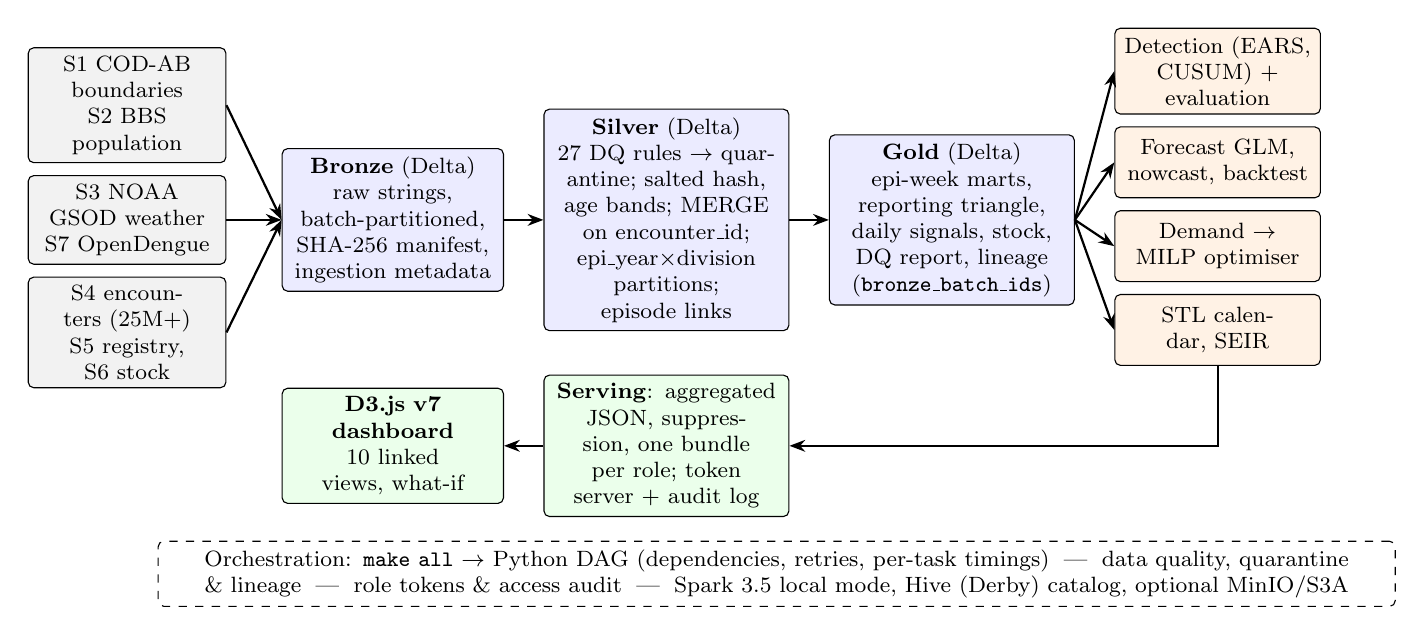
\begin{tikzpicture}[font=\footnotesize, box/.style={draw, rounded corners=2pt, align=center, minimum height=0.9cm, inner sep=3pt},
  src/.style={box, fill=gray!10, text width=2.3cm}, lay/.style={box, fill=blue!8, text width=2.9cm}, ana/.style={box, fill=orange!10, text width=2.4cm},
  arr/.style={-{Stealth[length=2mm]}, thick}]
\node[src] (s1) {S1 COD-AB boundaries\\S2 BBS population};
\node[src, below=0.15cm of s1] (s3) {S3 NOAA GSOD weather\\S7 OpenDengue};
\node[src, below=0.15cm of s3] (s4) {S4 encounters (25M+)\\S5 registry, S6 stock};
\node[lay, right=0.7cm of s3, text width=2.6cm] (b) {\textbf{Bronze} (Delta)\\raw strings, batch-partitioned, SHA-256 manifest, ingestion metadata};
\node[lay, right=0.5cm of b] (s) {\textbf{Silver} (Delta)\\27 DQ rules $\rightarrow$ quarantine; salted hash, age bands; MERGE on encounter\_id; epi\_year$\times$division partitions; episode links};
\node[lay, right=0.5cm of s] (g) {\textbf{Gold} (Delta)\\epi-week marts, reporting triangle, daily signals, stock, DQ report, lineage (\texttt{bronze\_batch\_ids})};
\node[ana, above right=0.25cm and 0.5cm of g] (d) {Detection (EARS, CUSUM) + evaluation};
\node[ana, below=0.15cm of d] (f) {Forecast GLM, nowcast, backtest};
\node[ana, below=0.15cm of f] (o) {Demand $\rightarrow$ MILP optimiser};
\node[ana, below=0.15cm of o] (c) {STL calendar, SEIR};
\node[box, fill=green!8, text width=2.9cm, below=0.55cm of s] (sv) {\textbf{Serving}: aggregated JSON, suppression, one bundle per role; token server + audit log};
\node[box, fill=green!8, text width=2.6cm, left=0.5cm of sv] (dash) {\textbf{D3.js v7 dashboard}\\10 linked views, what-if};
\draw[arr] (s1.east) -- (b.west); \draw[arr] (s3.east) -- (b.west); \draw[arr] (s4.east) -- (b.west);
\draw[arr] (b) -- (s); \draw[arr] (s) -- (g);
\foreach \n in {d,f,o,c} \draw[arr] (g.east) -- (\n.west);
\draw[arr] (c.south) |- (sv.east); \draw[arr] (sv) -- (dash);
\node[box, dashed, text width=15.5cm, minimum height=0.6cm, anchor=north] (orch) at ($(sv.south)+(1.4,-0.3)$) {Orchestration: \texttt{make all} $\rightarrow$ Python DAG (dependencies, retries, per-task timings) \;|\; data quality, quarantine \& lineage \;|\; role tokens \& access audit \;|\; Spark 3.5 local mode, Hive (Derby) catalog, optional MinIO/S3A};
\end{tikzpicture}
\caption{EpiScope architecture (medallion lakehouse + analytics + D3.js serving layer).}\label{fig:arch}
\end{figure*}

\subsection{Processing and storage}
All heavy work runs in PySpark 3.5 (\req{ING-2}); pandas appears only inside grouped UDFs on
per-district series and for final aggregated exports. Every layer is a \textbf{Delta Lake} table (Parquet
+ transaction log) registered in a Hive catalog backed by Derby (\req{ING-3}): \texttt{episcope\_bronze},
\texttt{\_silver} and \texttt{\_gold} databases. Delta gives ACID MERGE (idempotent upserts), \texttt{replaceWhere}
(recompute only affected epi-weeks) and time travel (\req{ING-7}). Setting \texttt{paths.lake\_root} to an
\texttt{s3a://} URI switches storage to MinIO through the S3A connector (\req{ING-5}; MinIO service in
\texttt{docker-compose.yml}).

\subsection{Partitioning}
Silver encounters are partitioned by \texttt{(epi\_year, adm1\_pcode)}: almost every query restricts the
period, and allocation and division dashboards restrict the division; 6 years $\times$ 8 divisions gives 48
directories whose files stay large (tens of MB) at SF\,=\,1. Partitioning by district would create 384
directories with many small files and skew (Dhaka alone holds a large share of the rows); by epi-week it
would create thousands of tiny files. Gold marts are small and partitioned by \texttt{epi\_year}; bronze is
partitioned by load batch so that silver reads exactly one batch.

\subsection{Cadence (C4) and streaming}\label{sec:cadence}
The operational cadence is a daily incremental batch (\texttt{make drop}); decisions it supports (weekly
forecasts, fortnightly shipments) do not need fresher data, and the batch is cheap. For emergencies a
Structured Streaming job (\req{ING-6}, \texttt{pipeline/streaming/stream\_alerts.py}) watches a file inbox and,
in each micro-batch, reuses the \emph{same} bronze/silver/gold code and detection, refreshing
\texttt{alerts.json}; the file-to-alert latency is logged (\S\ref{sec:evinc}).

\subsection{Reproducibility and orchestration}
\texttt{make all} creates a virtual environment from a fully pinned \texttt{requirements.txt}, writes a
git-ignored \texttt{.env} with a random salt and role tokens, and runs a small DAG runner
(\texttt{orchestration/dag.py}): tasks with dependencies, one fresh JVM per stage, retries with exponential
back-off and a JSON run record with per-task timings (\req{ENG-1}, \req{ENG-4}). A Dockerfile and
\texttt{docker-compose.yml} give the same result in containers. Nothing hard-codes dates, file names or row
counts: files are recognised by their header and the as-of date is the latest report date in silver.

\begin{table}[t]\centering\footnotesize
\caption{Alternatives considered}\label{tab:alt}
\begin{tabular}{@{}p{1.5cm}p{2.2cm}p{4.0cm}@{}}\toprule
Decision & Chosen & Alternative (why not)\\\midrule
Table format & Delta Lake & plain Parquet (no MERGE/time travel); Iceberg (heavier catalog set-up)\\
Storage & local FS / MinIO & HDFS in Docker (more RAM on a laptop)\\
Orchestration & Makefile + DAG runner & Airflow/Prefect (services and memory for a 6-task DAG)\\
Detection & CUSUM on historical limits & Farrington flexible (needs years of clean baseline per series; slower)\\
Forecast & per-district NB GLM & pooled HGB (more accurate, opaque, over-wide intervals: challenger); ARIMA (no count noise, weather lags awkward)\\
Optimiser & SciPy HiGHS MILP & PuLP/CBC (extra binary); heuristics (no optimality guarantee)\\
Serving & stdlib server + static JSON & database-backed API (not needed for $<$10\,MB of aggregates)\\\bottomrule
\end{tabular}\end{table}

% ================================================================================================ 4
\section{Data Generation, Quality, Lineage and Privacy}\label{sec:data}
\subsection{Public data (S1--S3, S7)}
District (ADM2, 64) and upazila (ADM3, 507) boundaries and centroids come from OCHA COD-AB v03 (HDX),
simplified to a 55\,kB TopoJSON for the browser; the OpenDengue V1.3 Bangladesh series~\cite{opendengue} checks
the synthetic seasonality. Because weather drives the synthetic epidemiology, S2 and S3 are \emph{pinned real
snapshots} committed in \texttt{data/reference}, so every clone generates the same data as this report (a
design decision: our build machine could not reach Open-Meteo, HDX or WorldPop, and a live download would
change every result). \textbf{Weather (S3)}: raw daily NOAA GSOD files~\cite{gsod} of \WxStations{} Bangladesh
Meteorological Department stations, stored unmodified and ingested as raw bytes; silver converts units, derives
relative humidity from dew point (Magnus formula) and interpolates to district centroids (inverse-distance
squared, four nearest stations within 150\,km). The mirror ends on \WxObservedUntil{}; the remaining
\WxFillPct{}\% of district-days use each district's day-of-year climatology of the same stations and are labelled
\texttt{climatology\_fill}. \textbf{Population (S2)}: Meta/CIESIN HRSL layers~\cite{hrsl} (total, men, women,
under-5, 15--24, 60+; about 12\,GB of 30\,m cells) summed on a 0.01$^\circ$ grid and assigned to the COD-AB
districts by point in polygon (\texttt{generator/build\_reference.py}); national total \PopTotalM{}\,M. The
5--14/25--44/45--64 split of the remaining ages uses stated fixed proportions (an assumption). Provenance
(\emph{real}, \emph{reference} or \emph{synthetic fallback}) is recorded per source and shown on the dashboard:
boundaries \ProvBound{}, weather \ProvWeather{}, population \ProvPop{}. \texttt{fetch\_public --refresh}
downloads Open-Meteo~\cite{openmeteo} and the HDX COD-PS census table instead where reachable.

\subsection{Synthetic encounter generator (S4--S6)}
\texttt{generator/generate.py} is parameterised by a scale factor and a seed and is deterministic: each
(district, year) chunk has its own \texttt{SeedSequence}, so output is byte-identical for any number of
worker processes (tested). At SF\,=\,1 it writes \GenRows{} encounter rows reported in 2021--2025 plus
\GenDropRows{} rows in 14 future daily drops, a registry of \GenFacilities{} facilities placed on real
upazilas (district hospitals, upazila health complexes, medical colleges, Dhaka-heavy private clinics) and
daily JSON stock and bed-occupancy snapshots. Expected daily counts per district and disease are:
dengue driven by 4--8-week lagged rainfall and 3--6-week temperature suitability, amplified in large cities;
diarrhoea with pre- and post-monsoon peaks and spikes 3--14 days after extreme rainfall; ILI with a
rainy-season and a winter peak; malaria concentrated in the hill districts. Counts are drawn from a
negative binomial (Poisson--gamma). We injected \GenOutbreaks{} outbreaks: 22 sharp local outbreaks of
different size and duration, 3 slow-growing ones, a 2023-like dengue epidemic in five cities, post-flood
cholera in Sylhet, two outbreaks that begin in the future drops, and a nationwide novel-respiratory surge
spreading from Dhaka with distance. Realism defects: $\approx$2\% resubmitted \texttt{encounter\_id}s,
0.5\% orphan facility keys, $\approx$1\% invalid values, a right-skewed 0--21-day reporting delay with fewer
reports on Fridays, Saturdays and holidays, a facility silent for 21 days that then back-fills, and a large
private network that starts reporting mid-stream. Truth files (outbreaks, artefacts, duplicate pairs) are
written to \texttt{data/ground\_truth}, which only the evaluation module reads (enforced by a test).

\subsection{Ingestion and incremental, idempotent loads}\label{sec:inc}
Bronze (\req{ING-1}) stores every row unmodified as strings plus \texttt{\_source, \_load\_ts, \_batch\_id,
\_file\_name, \_file\_checksum}; CSV columns are matched by name, so re-ordered or extra columns are tolerated.
The SHA-256 of every file is kept in a manifest, and a file already seen is skipped. Silver MERGEs on
\texttt{encounter\_id} (keeping the earliest report date as \texttt{first\_report\_date}); gold is recomputed
with \texttt{replaceWhere} from the Monday of the earliest onset week in the batch. Hence re-running a day
changes nothing and late records (up to 21 days, and back-filled ones beyond) update the epi-weeks they
belong to (\req{ING-4}); an integration test loads a drop, reloads it, force-reloads it and checks that silver
and gold are identical.

\subsection{Data quality (DQ-1, DQ-2, DQ-4)}\label{sec:dq}
27 rules are evaluated as Spark column predicates (16 on encounters: schema, IDs, referential integrity,
dates, onset$\leq$report, plausible delay, date range, age, sex, ICD-10 format and category, booleans, outcome,
geography; 6 on the registry; 5 on stock). A row failing any rule goes to \texttt{silver.quarantine} with all
its reason codes; the per-load report (rows in/out, quarantined, duplicates, pass rate per rule) is a gold
table and a dashboard view. In the SF\,=\,1 load \DqQuarantined{} of \DqRowsIn{} encounter rows
(\DqQuarPct{}) were quarantined and \DqDupRemoved{} resubmissions removed. Cross-facility duplicate visits
(\req{DQ-4}) are linked when the salted hash, disease group, sex and adjacent age band agree and onsets are
at most 7 days apart; against \DedupTrue{} injected duplicate pairs (3\% with a wrong sex, 30\% with a
mistyped age) precision was \DedupPrecision{} and recall \DedupRecall{}, and \DedupWrongMerge{} genuinely
separate episodes were merged.

\subsection{Lineage (DQ-3)}
Every gold row carries \texttt{bronze\_batch\_ids}, the sorted set of bronze batches whose records produced
it, and \texttt{gold.lineage\_batches} maps each batch to its files, checksums and row counts; a test checks
that every contributing batch exists in the manifest.

\subsection{Privacy by design (PRV-1..4)}\label{sec:privacy}
Patient IDs are replaced in silver by SHA-256(salt\,$\Vert$\,ID) with a salt that lives only in the
git-ignored \texttt{.env}; exact ages become six bands; the quarantine stores hashes too (\req{PRV-1}). The
browser receives only aggregates: primary suppression hides every count from 1 to 4, and complementary
suppression hides a second cell whenever a published district$\rightarrow$division$\rightarrow$national total
would reveal a single hidden cell (iterated to a fixed point); no totals across weeks or diseases are
published. An automated audit replays every exported hierarchy and scans every count field
(\req{PRV-2}). Role tokens select a bundle: national users see all districts, a district user sees their
district in detail and everything else only as division aggregates (\req{PRV-3}); each access is logged.
A k-anonymity check on a record-level research extract (\req{PRV-4}, Table~\ref{tab:kanon}) climbs a
generalisation ladder until $k\geq5$ with $\leq1\%$ suppression. For public releases we recommend
differential privacy instead: adding Laplace noise with scale $1/\varepsilon$ to weekly district counts
(sensitivity 1 per person-week) protects against linkage attacks that k-anonymity cannot stop, at the cost
of bias in small districts; $\varepsilon\approx1$ per released table and a privacy budget per year are
reasonable starting points.

\begin{table}[t]\centering\footnotesize
\caption{k-anonymity of a malaria research extract (k = 5)}\label{tab:kanon}
\begin{tabular}{@{}lrrrrc@{}}\toprule
Level & Records & Classes & $k_{\min}$ & Suppressed & $\leq$1\%\\\midrule
\tabinput{generated/kanon_table.tex}
\bottomrule\end{tabular}\\[2pt]
{\scriptsize L0 district$\times$week$\times$6 age bands$\times$sex; L1 month; L2 division; L3 3 age bands; L4 quarter.}
\end{table}

% ================================================================================================ 5
\section{Analytics Methods}\label{sec:methods}
\subsection{Outbreak detection (AN-1)}
Detection runs daily per district and disease on counts by first report date. The \emph{guarded} signal
excludes duplicate episodes and back-filled records (records reported on the first day a normally daily
facility reports again after $\geq$7 silent days, with delay $\geq$3 days); days on which more than 15\% of
the records come from a facility that started reporting in the last 56 days are flagged ``verify reporting''
rather than alerted. Weekday reporting effects are removed with national weekday factors.
\textbf{EARS C1/C2/C3} \cite{hutwagner2003} use Spark window functions: $z_t = (x_t-\bar x)/s$ over a 7-day
baseline (C2/C3 with a 2-day guard band; C3 sums positive C2 exceedances over 3 days), with
$s\geq\max(\sqrt{\bar x},0.5)$ for sparse series. The \textbf{seasonal CUSUM} runs in a grouped pandas UDF:
the expected 7-day count is the historical limit \cite{stroup1989} (mean of the same window $\pm$2 weeks in
each earlier year) multiplied by this year's level over the last 2--7 weeks (2-week guard band), the daily
count is standardised by $\sqrt{\mu\hat\phi}$ with a prospective quasi-Poisson dispersion $\hat\phi$ (mean
squared Pearson residual over the past year, winsorised), and $C_t=\max(0, C_{t-1}+z_t-0.5)$ \cite{page1954}.
An alert also needs at least \MinCount{} cases in the last 7 days.

\subsection{Forecasting and nowcasting (AN-4)}
For every district and disease and each horizon $h\in\{1..4\}$ weeks, a direct log-linear Poisson model
(ridge $\lambda=0.02$) uses the last two weeks (log), the mean of weeks $t-5..t-2$, the same season last
year, annual harmonics of the target week, rainfall summed and temperature averaged over weeks
$t+h-8..t+h-4$ (the 4--8-week lag), and the recent maximum daily rainfall. A negative-binomial size
estimated by moments gives predictive quantiles. The 256 series are trained in parallel with
\texttt{groupBy(district, disease).applyInPandas}. Because the last 3--4 weeks are incomplete, the counts
known at the origin are rebuilt from the reporting triangle (onset week$\times$report week) and divided by
the national completeness at that delay, estimated only from weeks 8--60 weeks before the origin. Baseline:
seasonal naive (same week last year) with empirical error quantiles; comparator: gradient-boosted trees
pooled over districts on $\log(1+y)$.

\subsection{Demand conversion (AN-6)}
Weekly case quantiles are sampled (1{,}000 Monte-Carlo draws by inverse-CDF interpolation), admissions are
binomial with the district's admission rate over the last 52 weeks shrunk to the national rate (50
pseudo-cases), and converted with stated assumptions: 6 bags of IV saline per admitted dengue case and 8 per
admitted diarrhoea case (+0.3 per outpatient diarrhoea case), 1.3 NS1 kits per suspected dengue case, 10 ORS
sachets per diarrhoea case, 1 artemisinin course per malaria case, and length of stay 3--5 days for bed-days.
The mean and 10/50/80/90\% quantiles over 4 weeks are kept.

\subsection{Allocation optimiser (AN-7)}
With $\hat y_{d,r}$ the 80th percentile of demand, $s_{d,r}$ the latest stock, $c_r$ unit cost, $p_d$
population share and $w_d = 1 + [\text{alert}] + 0.5[\text{forecast growth}>20\%]$:
\begin{align*}
\min\;& \textstyle\sum_{d,r} w_d h_r (u_{d,r}+\beta q_{d,r}) + \sum_d w_d H_T v_d + \epsilon\sum_{d,r} c_r x_{d,r}\\
\text{s.t. }& u_{d,r}\geq \hat y_{d,r}-s_{d,r}-x_{d,r},\quad q_{d,r}\geq u_{d,r}-g_{d,r}/2,\\
& \textstyle\sum_{d,r} c_r x_{d,r}\leq B,\\
& x_{d,r}\geq \alpha p_d \textstyle\sum_{d'} x_{d',r},\quad \sum_{d\in k}\sum_r m_r x_{d,r}\leq T_k,\\
& v_d\geq \tau_d - z_d,\; \textstyle\sum_d z_d\leq N,\; z_d\in\mathbb Z_{\geq0},\; x,u,v\geq0.
\end{align*}
Unmet units are valued in patient-equivalents $h_r$ = share of one patient's need a unit covers $\times$ a
severity weight (life-threatening 3, severe 2, moderate 1, diagnostic 0.3): IV bag $\tfrac16\times3=0.5$, ACT
course $1\times2=2$, ORS sachet $\tfrac1{10}\times1=0.1$, NS1 kit $\tfrac1{1.3}\times0.3=0.23$; a missing team
$H_T=20$. These weights must be agreed with clinicians; they make sachets, kits and courses commensurable. The part of a shortfall beyond half of the district's gap $g_{d,r}$ costs $(1+\beta)$ times more
($\beta=1$): the first half of every gap -- the life-saving minimum -- is filled first. This convex penalty also
removes a degeneracy we observed: with purely linear valuation every taka has the same value in every district,
and the solver split ties arbitrarily (a high-need district could get nothing). $\tau_d$ is the number
of diseases alerting in district $d$ (rapid-response team demand, $N=20$ teams); $m_r$ are unit weights and
$T_k$ a truck-capacity limit per division. $\alpha$ is the policy lever of conflict C3: the guaranteed
fraction of each district's population share of every resource shipped. The MILP ($\approx$640 variables) is
solved with HiGHS \cite{huangfu2018} in well under a second. Baseline: the same budget split across resources
by national gap and across districts by population.

\subsection{Preparedness calendar (AN-9)}
Weekly counts per division and disease are decomposed with robust STL \cite{cleveland1990} (period 52, log
scale) in a grouped UDF; the seasonal component averaged by ISO week gives a multiplicative seasonal index.
The season is the longest circular run of $\geq$3 weeks with index $\geq1.15$; campaigns start 8 weeks
(dengue larval control), 6 (malaria) or 4 weeks before onset, supplies are pre-positioned 4 weeks before
onset and staff surge 2 weeks before the peak, projected onto the next 52 weeks.

\subsection{Epidemic scenarios (AN-10)}
The novel-respiratory surge is located from data alone (national ILI above 130\% of the same-week median of
other years). A deterministic SEIR model (latent 3 days, infectious 5 days) is fitted to the weekly excess by
least squares on the square-root scale (free: $\beta$, $I_0$, reporting fraction $\rho$), giving
$R_0=\SeirRzero{}$, $\rho=\SeirRho{}$ and $R^2=\SeirRtwo{}$. What-if scenarios reduce $\beta$ by 20\% or 40\%
from the detection week, two weeks earlier or later (Table~\ref{tab:seir}).

% ================================================================================================ 6
\section{Evaluation}\label{sec:eval}
All results are from the SF\,=\,1 build (\GenRows{} encounters), evaluated prospectively over
\EvalStart{}--\EvalEnd{} (the first year is the baseline burn-in).

\subsection{Detection (AN-2, AN-3, C1)}\label{sec:evdet}
Definitions: an outbreak (district$\times$disease) is detected if an alert falls between 3 days before its
start and 7 days after its end; days to detection count from the start; an \emph{alert event} is a run of
consecutive alert days, false if it overlaps no outbreak window. Local outbreaks (\NOutbreakRows{} rows
including the 64 district rows of the national surge) and the surge are reported separately.
Fig.~\ref{fig:tradeoff} and Table~\ref{tab:tradeoff} give the trade-off. At the chosen operating point
\OpMethod{}\,$\geq$\,\OpThreshold{} the pipeline detects \SensLocal{} of local outbreaks with a median of
\MedDelayLocal{} days after onset at \FAperDY{} false alerts per district-year (all four diseases together),
and flags \SensNRS{} of districts in the national surge (median \MedDelayNRS{} days).
\textbf{Reporting artefacts (AN-3).} In the back-fill district and window the naive signal produced
\ArtBackfillNaive{} alert days against \ArtBackfillGuarded{} for the guarded pipeline; around the onboarding
facility, \ArtOnboardNaive{} vs \ArtOnboardGuarded{} at the operating point (at lower thresholds the new-facility
flag routes such days to ``verify reporting'' instead of ``alert'').
\textbf{Interpretation.} The seasonal CUSUM dominates the EARS family everywhere on the curve: at a comparable
false-alert burden (at most 3.5 per district-year) EARS C1 finds \EarsCOneSensLowFA{}, C2 \EarsCTwoSensLowFA{} and C3
\EarsCThreeSensLowFA{} of local outbreaks, CUSUM \CusumSensLowFA{}. EARS compares a day with the previous week only, so every seasonal upswing and every post-flood spike looks
anomalous; CUSUM compares with the same season in earlier years and accumulates small persistent excesses. The
price is delay: \MedDelayLocal{} days at the operating point versus \CusumDelayHighFA{} days at thresholds that produce
10--20 false alerts per district-year -- this is conflict C1 in numbers, and the what-if slider lets
epidemiologists move along it. The national surge is detected in every district, but late relative to its
injected start (\MedDelayNRS{} days): the start is defined as the day seeding began, when only a few infections
per million existed, so the first weeks carry no visible excess. Three design errors were found and fixed by
this evaluation (AI\_USAGE.md): a too-narrow level adjustment that saturated CUSUM in epidemic years, CUSUM
increments computed on overlapping 7-day sums (strongly autocorrelated, which inflates false alerts), and a
median-based dispersion estimate that under-estimated variance.

\begin{figure}[t]\centering
\begin{tikzpicture}\begin{axis}[width=\columnwidth, height=5.2cm, xlabel={False alerts per district-year}, ylabel={Sensitivity (local)},
  ymin=0, ymax=1.02, xmin=0, xmax=12, restrict x to domain=0:12, legend pos=south east, legend style={font=\scriptsize}, tick label style={font=\scriptsize}, label style={font=\footnotesize}, grid=major, grid style={gray!20}]
\addplot+[orange, mark=square*, mark size=1.5pt, thick] table[col sep=comma, x=false_alerts_per_district_year, y=sensitivity_local] {generated/tradeoff_earsc1.csv};
\addplot+[teal, mark=triangle*, mark size=1.7pt, thick] table[col sep=comma, x=false_alerts_per_district_year, y=sensitivity_local] {generated/tradeoff_earsc2.csv};
\addplot+[olive, mark=diamond*, mark size=1.7pt, thick] table[col sep=comma, x=false_alerts_per_district_year, y=sensitivity_local] {generated/tradeoff_earsc3.csv};
\addplot+[blue, mark=*, mark size=1.5pt, very thick] table[col sep=comma, x=false_alerts_per_district_year, y=sensitivity_local] {generated/tradeoff_cusum.csv};
\legend{EARS C1, EARS C2, EARS C3, CUSUM}
\end{axis}\end{tikzpicture}
\caption{Detection trade-off (guarded pipeline), one point per threshold.}\label{fig:tradeoff}
\end{figure}

\begin{table}[t]\centering\footnotesize
\caption{Detection over the threshold grid (* = operating point)}\label{tab:tradeoff}
\begin{tabular}{@{}lrrrrrr@{}}\toprule
Method & Thr. & Sens. & Delay & FA/DY & FA naive & NRS\\\midrule
\tabinput{generated/tradeoff_table.tex}
\bottomrule\end{tabular}\\[2pt]
{\scriptsize Delay = median days to detection; FA/DY = false alert events per district-year (4 diseases); NRS = share of districts detecting the national surge.}
\end{table}

\subsection{Forecasting backtest (AN-5, C5)}\label{sec:evfc}
Rolling-origin backtest over the last 52 complete weeks (models refitted every 4 origins on data complete at
the origin; nowcast inputs), scored on identical cells for all models (Table~\ref{tab:fc}). Averaged over all
districts and diseases, the GLM's one-week-ahead MAE is \GlmMAEOne{} vs \BaseMAEOne{} for the seasonal naive
and \HgbMAEOne{} for pooled boosting; its WIS is \GlmRelWISOne{} of the baseline's at one week and
\GlmRelWISFour{} at four weeks, and 80\% intervals cover \GlmCovOne{} (h\,=\,1) and \GlmCovFour{} (h\,=\,4) of
outcomes, close to the nominal 80\% (seasonal naive: \BaseCovOne{}). Skill decays with horizon as expected;
the largest gains are for ILI and dengue, whose weather-driven and multi-year patterns the naive method cannot
follow. The pooled boosted model is more accurate at all horizons (relative WIS \HgbRelWISOne{} at $h=1$,
\HgbRelWISFour{} at $h=4$), because it shares information across districts, but its intervals over-cover
(\HgbCovOne{} at $h=1$) and it cannot be explained district by district; we keep the GLM for decisions (C5) and
log the challenger, whose accuracy advantage is the main argument for a hierarchical model in future work.

\begin{table}[t]\centering\footnotesize\setlength{\tabcolsep}{3pt}
\caption{Backtest (last 52 weeks): MAE, 80\% coverage, WIS relative to seasonal naive}\label{tab:fc}
\begin{tabular}{@{}lrrrrrrrr@{}}\toprule
Disease & h & \multicolumn{3}{c}{MAE: naive / GLM / HGB} & Cov$_{\text{naive}}$ & Cov$_{\text{GLM}}$ & rWIS$_{\text{GLM}}$ & rWIS$_{\text{HGB}}$\\\midrule
\tabinput{generated/forecast_table.tex}
\bottomrule\end{tabular}\end{table}

\subsection{Allocation vs.\ baseline and equity (AN-7, AN-8, C3)}\label{sec:evopt}
With stock on \StockDate{}, closing every district's gap at the planning quantile would cost
\FullGapBDT{}\,M BDT; at a budget of 60\% of that (\BudgetBDT{}\,M) the optimised plan with $\alpha=\AllocAlpha{}$
leaves weighted unmet need of \OptWUnmet{} vs \BaseWUnmet{} patient-equivalents for the population-proportional plan,
covers \OptGapCov{}\% vs \BaseGapCov{}\% of the gap, and leaves \OptBelowHalf{} vs \BaseBelowHalf{} districts
below half coverage; unmet rapid-response team demand is \OptTeamsUnmet{} vs \BaseTeamsUnmet{} teams.
Table~\ref{tab:equity} gives the efficiency--equity curve over six budgets. Rule: take the smallest $\alpha$ that
leaves no district with a gap and nothing shipped, provided it costs at most 10\% extra weighted unmet demand
against the purely efficient plan; at 60\% budget this gives $\alpha=\RecAlpha{}$ (loss \RecEffLoss{}\%,
districts left with nothing \RecNothingZero{}$\rightarrow$\RecNothing{}).
\textbf{Interpretation.} In this low-season snapshot (end of December) the shortfall is almost entirely ORS and
IV saline; per taka, ORS protects about four times more patient-equivalents than IV saline, so the plan first
closes ORS gaps everywhere, then IV saline where alerts or growth raise the weight. Population-proportional
allocation spends the same money but ships saline and sachets to districts that already hold enough, which is
why it meets less than half as much of the gap. Every extra step of $\alpha$ costs efficiency with diminishing
equity gains (Table~\ref{tab:equity}); a small floor ($\alpha=\RecAlpha{}$) is enough to guarantee every
district a share, and larger values mostly move supplies from districts with a gap to districts without one.

\begin{table}[t]\centering\footnotesize\setlength{\tabcolsep}{3.5pt}
\caption{Efficiency--equity curve (weighted unmet need in patient-equivalents; coverage valued at cost)}\label{tab:equity}
\begin{tabular}{@{}llrrrr@{}}\toprule
Budget & Plan & W.\ unmet & Gap cov.\ \% & Min cov. & $<$50\%\\\midrule
\tabinput{generated/equity_table.tex}
\bottomrule\end{tabular}\end{table}

\subsection{Scalability and Spark optimisations (ENG-2, ENG-3)}\label{sec:evperf}
Table~\ref{tab:scale} reports the full \texttt{make all} (generator, load, analytics, export) at three scale
factors on \ScaleCpus{} vCPUs and \ScaleMem{}\,GB RAM (Spark local mode, 6\,GB heap, Java 17): SF\,=\,1 finishes in
\ScaleMinC{} minutes, well inside the 45-minute limit. Time grows roughly linearly with rows in the load stage,
while analytics is almost constant because it works on weekly/daily aggregates whose size depends on districts
and weeks, not on encounters. The Spark UI shows the silver stage as the bottleneck: it evaluates 16 rules,
hashes every patient ID, shuffles once by \texttt{encounter\_id} for resubmission handling and writes 48 partitions;
the next step would be to fold the per-rule statistics into the write job instead of separate actions.

\begin{table}[t]\centering\footnotesize\setlength{\tabcolsep}{2.2pt}
\caption{Scalability: seconds per stage, total minutes, data size (GB; the SF\,=\,1 lake also holds the Delta versions of three later incremental loads)}\label{tab:scale}
\begin{tabular}{@{}rrrrrrrrrrr@{}}\toprule
SF & Rows & Gen. & Bronze & Silver & Gold & Analyt. & Export & Total & Landing & Lake\\\midrule
\tabinput{generated/scaling_table.tex}
\bottomrule\end{tabular}\end{table}

Two optimisations with before/after evidence (median of three runs on the SF\,=\,1 lake, Spark UI screenshots in
\texttt{docs/experiments/screenshots}): (i) \textbf{broadcast join of the facility registry} -- with broadcasting
disabled Spark plans a SortMergeJoin that shuffles all \GenRows{} bronze encounters (Fig.~\ref{fig:sparkui}) and sorts both
sides; broadcasting the \GenFacilities{}-row registry gives a BroadcastHashJoin with no shuffle of the large side:
\OptBcastBefore{}\,s $\rightarrow$ \OptBcastAfter{}\,s (\OptBcastSpeedup{}$\times$); (ii) \textbf{columnar storage} --
the same per-facility, per-diagnosis count over all encounters reads \OptColCsvGB{}\,GB of CSV in the landing zone
but only two of 17 columns from \OptColParquetGB{}\,GB of zstd Parquet in bronze: \OptColBefore{}\,s
$\rightarrow$ \OptColAfter{}\,s (\OptColSpeedup{}$\times$). (iii) \textbf{Partition pruning} on silver
(epi\_year$\times$division) cuts the files scanned by a division-year query from \OptPruneFilesBefore{} to
\OptPruneFilesAfter{}, but the wall-time gain is small at this size (\OptPruneBefore{}\,s $\rightarrow$
\OptPruneAfter{}\,s) because the table is already in the operating-system cache; it grows with data volume.
Adaptive query execution (skew-join handling, coalescing of the 32 shuffle partitions) is enabled throughout;
we did not run a separate skew experiment.

\begin{figure*}[t]\centering
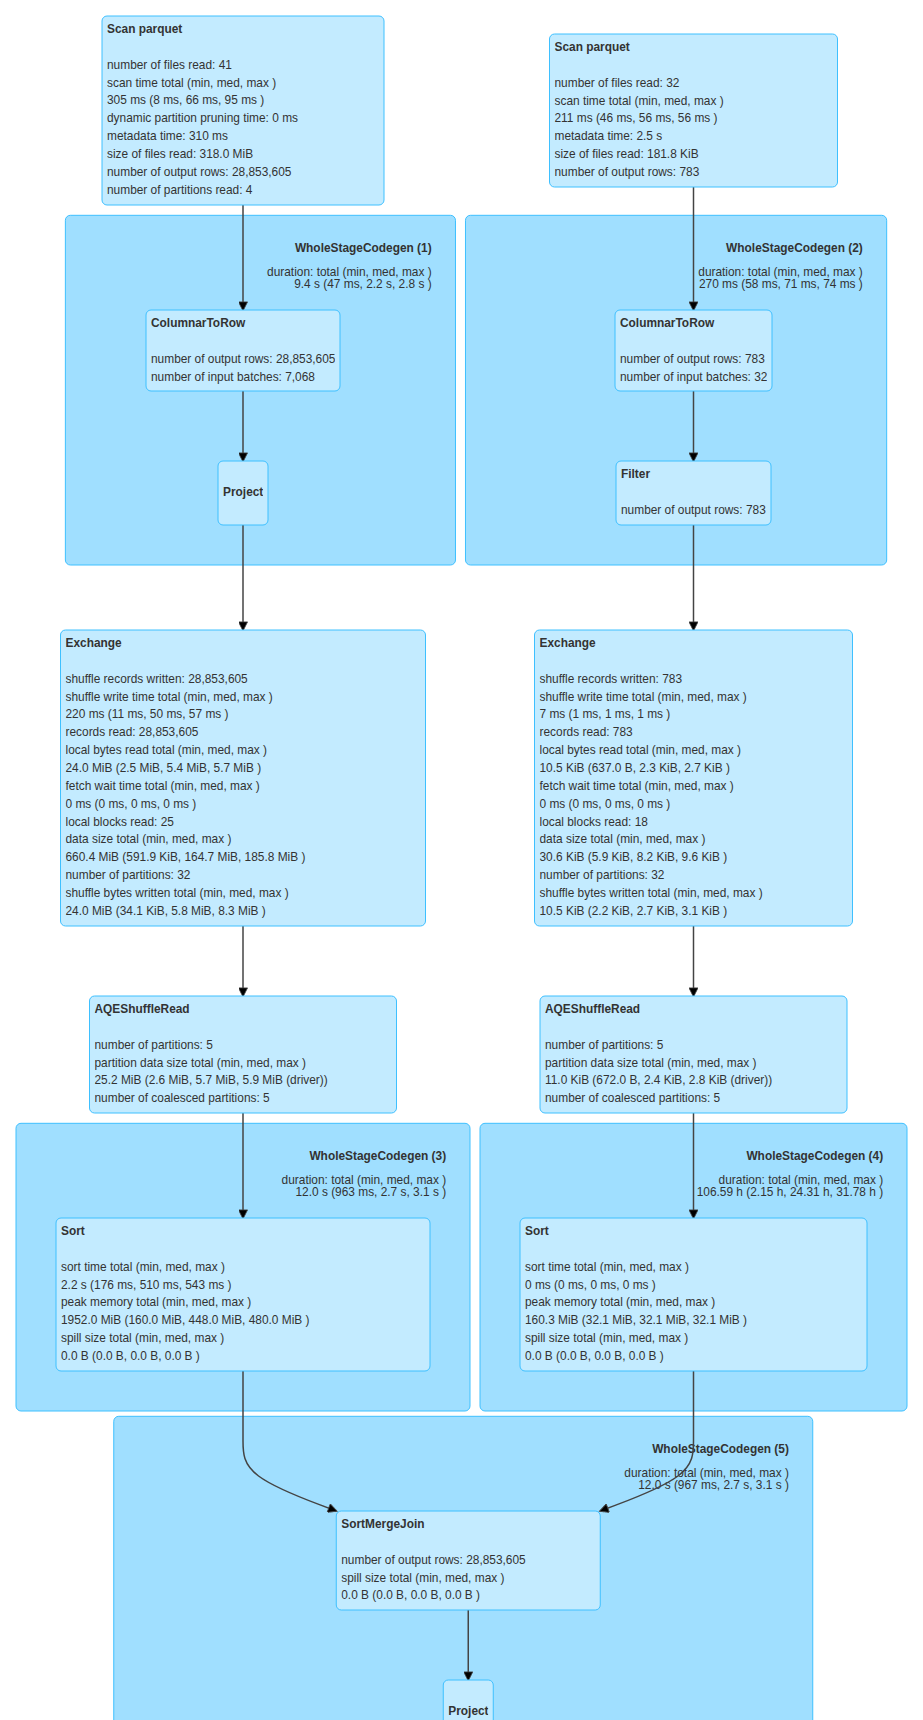
\includegraphics[width=0.49\textwidth,height=8cm,keepaspectratio]{spark_ui_broadcast_off.png}\hfill
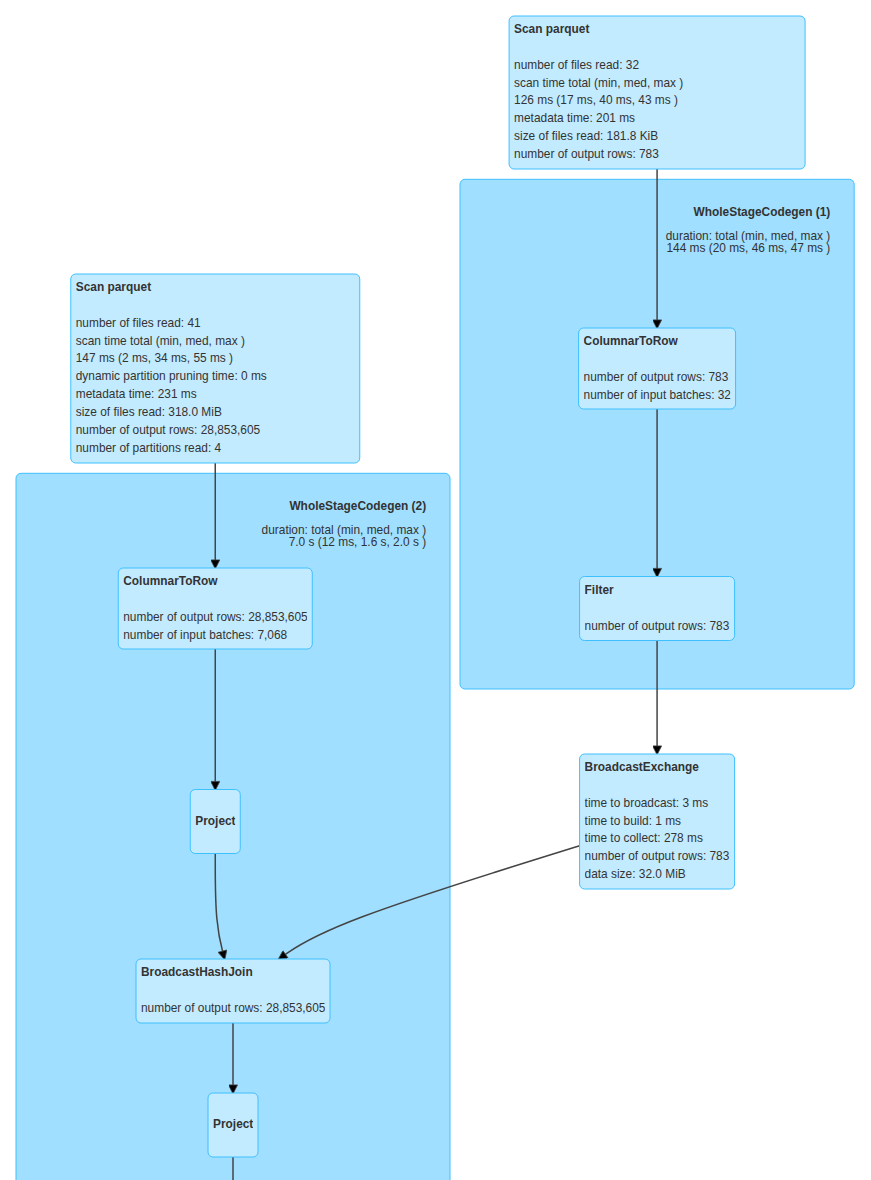
\includegraphics[width=0.49\textwidth,height=8cm,keepaspectratio]{spark_ui_broadcast_on.png}
\caption{Spark UI (History Server, SQL tab) for the registry join on the SF\,=\,1 lake. Left: broadcast disabled --
both sides are shuffled (Exchange) and sorted before a SortMergeJoin. Right: BroadcastHashJoin -- the small facility
registry is broadcast and the encounters are joined where they are read, with no shuffle of the large side.}
\label{fig:sparkui}
\end{figure*}

\subsection{Incremental loads, streaming and calendar}\label{sec:evinc}
\textbf{Incremental and idempotent (\req{ING-4}).} Loading the first future daily drop into the SF\,=\,1 lake added
\IncNewRows{} encounters (including late records whose onsets fall in earlier epi-weeks) in \IncLoadSec{}\,s, and
the whole drop DAG including analytics and dashboard export took \IncDagMin{} minutes. Re-running the same day
returned ``nothing new'' in \IncRerunSec{}\,s; a forced re-ingest (\IncForceSec{}\,s) left silver at \IncSilverRows{} rows, all
with distinct \texttt{encounter\_id}, and every gold count unchanged. \textbf{Hidden-drop rehearsal.} Pointing
\texttt{make drop} at the folder with all 14 generated days (same schema, new outbreaks, quality defects)
skipped the day already loaded and ingested the other \RehDays{} days (\RehRows{} rows, \RehQuar{} quarantined)
in \RehMin{} minutes end to end, regenerating alerts, forecasts, allocation and dashboard data without any code
change. \textbf{Streaming (\req{ING-6}).} With the Structured Streaming job running (30-second trigger), a new
encounter file dropped in the inbox refreshed \texttt{alerts.json} after a median of \StreamLatencyMed{}\,s
(maximum \StreamLatencyMax{}\,s), inside the 5-minute requirement. \textbf{Time travel (\req{ING-7}).} Every
load creates a new Delta version of silver and gold, so ``what did we know on day $t$'' is a
\texttt{versionAsOf} read (\texttt{make inspect WHAT=asof}). Reading \texttt{gold.weekly\_counts} at the version
before the rehearsal drop shows the counts known on \TTKnownUntil{}; the drop's late reports revised
\TTRevisedWeeks{} of the \TTRows{} recent disease-weeks. The backtest does not keep a version per day: it rebuilds
past knowledge from report dates (the reporting triangle). Rebuilding the same weeks from today's silver with
\emph{first report date $\leq$ \TTKnownUntil{}} differs from the time-travel read by \TTTriangleDiff{} of
\TTKnownThen{} cases, which validates that shortcut.
Table~\ref{tab:cal} shows the dengue calendar for the next 12 months.

\begin{table}[t]\centering\footnotesize\setlength{\tabcolsep}{3pt}
\caption{Dengue preparedness calendar (next 12 months)}\label{tab:cal}
\begin{tabular}{@{}lrrrrr@{}}\toprule
Division & Campaign & Pre-position & Onset & Peak & End\\\midrule
\tabinput{generated/calendar_table.tex}
\bottomrule\end{tabular}\end{table}

\begin{table}[t]\centering\footnotesize\setlength{\tabcolsep}{3pt}
\caption{SEIR what-if scenarios for the respiratory surge}\label{tab:seir}
\begin{tabular}{@{}p{3.6cm}rrrr@{}}\toprule
Scenario & Reported & Peak wk & Peak & Averted\\\midrule
\tabinput{generated/seir_table.tex}
\bottomrule\end{tabular}\end{table}

% ================================================================================================ 7
\section{Dashboard Design and Usability}\label{sec:vis}
The dashboard (\req{VIS-1}) is plain HTML with D3.js v7 and topojson-client, vendored so it runs offline, and is
started with one command (\texttt{run\_dashboard.bat}, \texttt{./run\_dashboard.sh} or \texttt{make serve}), which
opens the browser already signed in. Fig.~\ref{fig:dash} shows the national view.

\textbf{Coordinated views (\req{VIS-2}, \req{VIS-3}).} (1) District choropleth of mean weekly incidence per
100{,}000 over the selected weeks with alert markers; (2) focus+context time series with the reported counts,
the nowcast for weeks still being reported, forecast median with 50/80/90\% bands and the alert threshold
(expected 7-day count + 2\,SD); (3) seasonal heatmap, epi-week$\times$year; (4) allocation view comparing forecast
demand (10--90\% interval and planning quantile), stock, recommended and baseline shipments; (5) ranked
early-warning table; plus the what-if panel, the preparedness calendar, SEIR scenarios, the per-load data-quality
report and an evaluation panel showing the detection trade-off and forecast skill. One shared state (disease,
area, week range, resource, threshold, budget, $\alpha$) is broadcast to every view with \texttt{d3.dispatch}:
clicking a district on the map, a row in the table or a bar in the allocation view selects it everywhere;
brushing the context strip or clicking a heatmap cell sets the period of the map and heatmap. Every view has
tooltips, legends and axis labels.

\textbf{Scale-aware design (\req{VIS-4}).} The browser loads only the role's bundle of aggregated JSON: the
national bundle is about 1.8\,MB plus a 55\,kB TopoJSON (limit 10\,MB, checked by a test). Counts are at
district$\times$epi-week (the level at which district officers act and stocks are managed); forecasts, demand and
allocations are per district for four weeks; detection is published as daily \emph{statistics} for the last
180 days so the threshold can be changed in the browser without shipping counts.

\textbf{What-if panel (\req{VIS-5}).} Sliders for budget (20--120\% of the gap), alert threshold and equity floor
$\alpha$ look up a precomputed grid of optimiser runs (every combination solved offline, because the alert
threshold changes the weights and team demand) and recompute alert status from the published statistics; the
efficiency--equity curve highlights the current $\alpha$.

\textbf{Accessibility and honesty (\req{VIS-6}).} Disease colours use a validated colour-blind-safe order (blue,
orange, aqua, yellow; adjacent CVD $\Delta E\geq9$ in both light and dark mode, checked with a palette
validator), magnitudes use a one-hue blue ramp, alert states use reserved status colours always paired with an
icon and a label; suppressed cells are hatched and shown as ``$<$5''; every forecast carries its bands; every
panel shows its data-freshness date and a banner states that the data are synthetic, the provenance of the
public inputs and until when the weather is observed rather than climatology. \textbf{Mobile and playback (\req{VIS-7}).} The grid collapses to one column below 1{,}100\,px and a
``Play spread'' button animates weekly incidence over the last year. \textbf{Roles (\req{PRV-3}).} A district
officer's token returns a bundle with their own district in detail and all other areas as division aggregates.
A ``View as'' menu switches role in the local demo mode; \texttt{--secure} turns off automatic sign-in.

\textbf{Usability check.} \todo{The protocol in \texttt{docs/usability/usability\_protocol.md} (six tasks, think-aloud,
System Usability Scale) must be run with at least two non-CS users; insert their results and the changes made here.}

\begin{figure*}[t]\centering
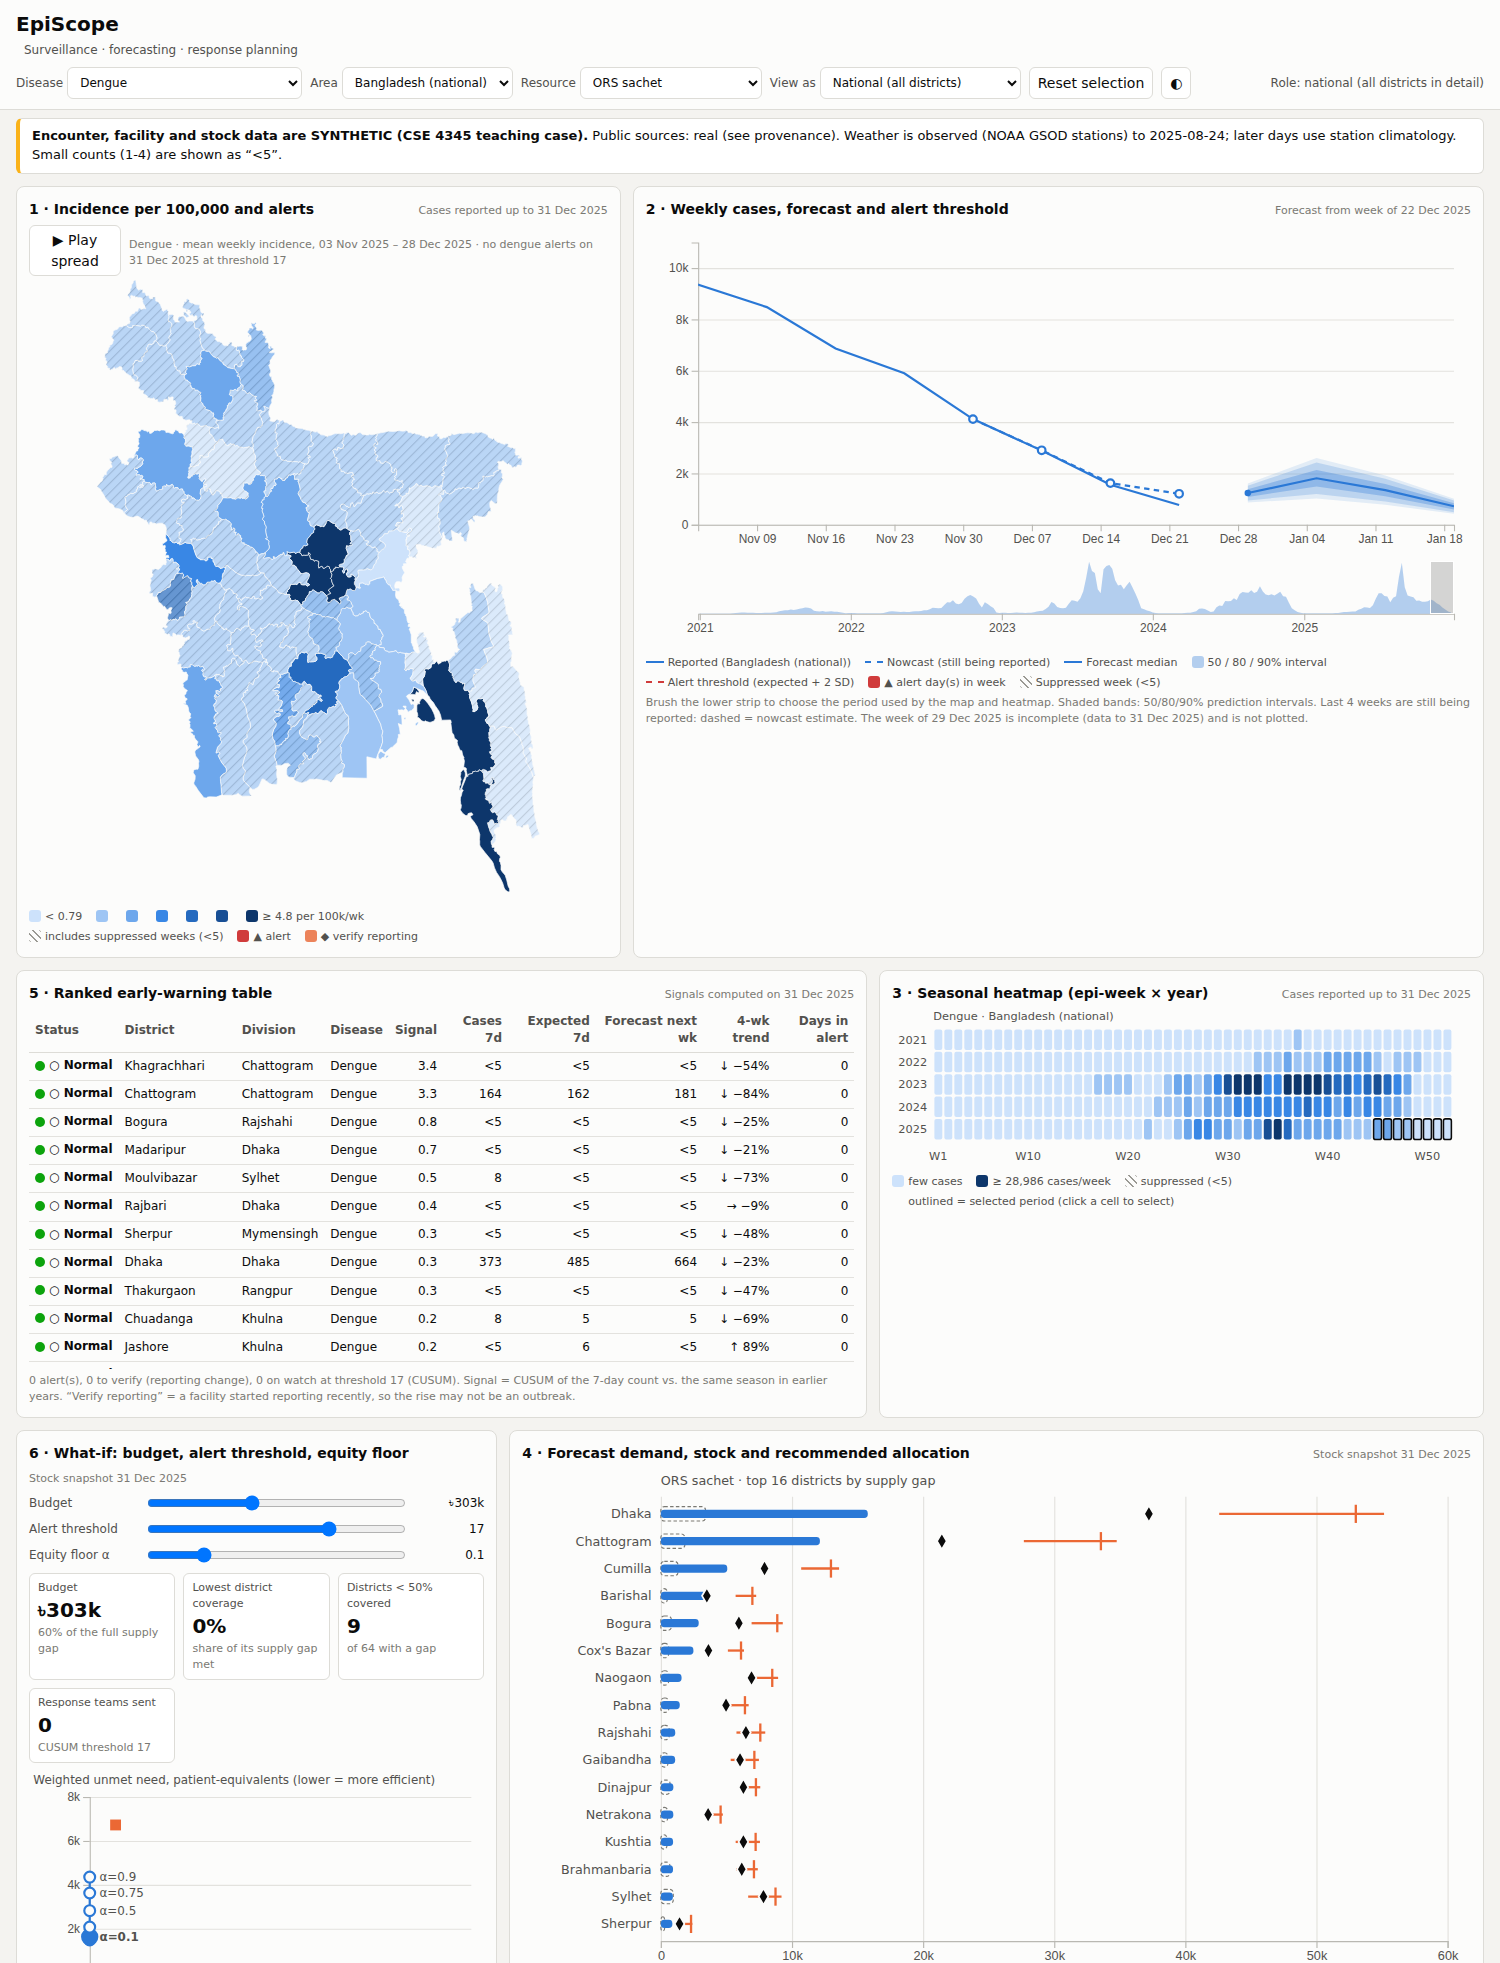
\includegraphics[width=0.92\textwidth]{dashboard_national.png}
\caption{EpiScope dashboard, national role (SF\,=\,1 build). Views are linked: selecting a district on the map
updates the time series, heatmap, table and allocation view.}\label{fig:dash}
\end{figure*}

% ================================================================================================ 8
\section{Ethical, Societal and Sustainability Considerations}\label{sec:ethics}
\textbf{Consequences of errors (A4).} A missed outbreak costs lives; a false alarm costs money and, repeated, the
trust that makes officials act on the next alert. We therefore report both error types, choose the operating
point openly, route reporting-artefact alerts to ``verify reporting'' instead of ``alert'', and recommend that
every alert is confirmed with the district before teams move. \textbf{Privacy.} The design follows
minimisation and purpose limitation: identifiers stop at bronze, salted hashes cannot be reversed without a key
that never enters the repository, exact ages are dropped, and the public-facing layer contains only suppressed
aggregates; stigma is a real risk for small communities (e.g.\ malaria in hill districts), which is why small
counts are hidden even at district level and why we recommend differential privacy for public releases.
\textbf{Equity.} Allocating purely on expected unmet need concentrates supplies in Dhaka and the hill districts;
the equity floor makes the trade-off explicit and gives policymakers a number to defend (``every district gets at
least $\alpha$ of its population share''). Weights for alerts and growth are stated and adjustable; they must be
agreed with the Ministry rather than set by engineers. \textbf{Misuse.} Alerts could be used to blame districts or
facilities; the dashboard shows reporting context (back-fills, new facilities) to avoid penalising good reporting,
and access is role-based and audited. \textbf{Automation bias.} Forecasts and plans are advisory: uncertainty
bands, the baseline plan and the what-if panel invite human judgement; the model is interpretable by design (C5).
\textbf{Sustainability.} The whole platform runs on one laptop-class machine in about \DagMinutes{} minutes per
full rebuild and a few minutes per daily increment, uses open-source software only, stores data compressed
(zstd Parquet) and recomputes only affected epi-weeks, keeping energy and cost low enough for district
infrastructure; the same code scales out to a cluster or object store without changes.
\textbf{Honesty about data.} Synthetic data can make methods look better than they will be on real reports
(cf.\ the Google Flu lesson \cite{lazer2014}); all results must be re-validated on Ministry data.

% ================================================================================================ 9
\section{Limitations and Future Work}\label{sec:limits}
(1) \emph{Synthetic data.} Outbreak shapes, delays and artefacts follow our own generator, so detection and
forecast accuracy are optimistic; validation on historical DGHS surveillance data (e.g.\ the 2019 and 2023
dengue seasons) is the first next step. Weather after \WxObservedUntil{} is station climatology (end of the NOAA
mirror), and three of six age bands use an assumed split; the census table and Open-Meteo can replace both.
(2) \emph{Detection.} Weather-driven genuine rises (post-flood diarrhoea, early dengue seasons) count as false
alerts against a ground truth that lists only injected outbreaks; a covariate-adjusted baseline (e.g.\ the
forecast GLM's residuals) and Farrington-flexible \cite{farrington1996} are natural extensions; slow outbreaks
are partly absorbed by the adaptive level. (3) \emph{Forecasting.} Direct models are refitted every four weeks,
features at training time use complete data while prediction uses nowcasts, and intervals assume independent
weeks. (4) \emph{Optimisation} is single-period with linear costs; multi-period stock dynamics, lead times,
cold-chain constraints and uncertainty (stochastic or robust programming) are future work. (5) \emph{Privacy.}
Complementary suppression protects the published hierarchy but not arbitrary external data; formal
differential privacy is recommended for public releases. (6) \emph{Engineering.} Local-mode Spark on one node;
HDFS/Kubernetes deployment, upazila-level maps with stronger suppression, SMS alerts to district officers and
integration with DHIS2 APIs are future work.

\bibliographystyle{IEEEtran}
\begin{thebibliography}{99}
\bibitem{hutwagner2003} L. Hutwagner, W. Thompson, G. M. Seeman, T. Treadwell, ``The bioterrorism preparedness and response Early Aberration Reporting System (EARS),'' \emph{J. Urban Health}, 80(1), 2003.
\bibitem{farrington1996} C. P. Farrington, N. J. Andrews, A. D. Beale, M. A. Catchpole, ``A statistical algorithm for the early detection of outbreaks of infectious disease,'' \emph{J. R. Stat. Soc. A}, 159(3), 1996.
\bibitem{stroup1989} D. F. Stroup, G. D. Williamson, J. L. Herndon, J. M. Karon, ``Detection of aberrations in the occurrence of notifiable diseases surveillance data,'' \emph{Stat. Med.}, 8(3), 1989.
\bibitem{page1954} E. S. Page, ``Continuous inspection schemes,'' \emph{Biometrika}, 41(1/2), 1954.
\bibitem{bracher2021} J. Bracher, E. L. Ray, T. Gneiting, N. G. Reich, ``Evaluating epidemic forecasts in an interval format,'' \emph{PLoS Comput. Biol.}, 17(2), 2021.
\bibitem{lazer2014} D. Lazer, R. Kennedy, G. King, A. Vespignani, ``The parable of Google Flu: traps in big data analysis,'' \emph{Science}, 343(6176), 2014.
\bibitem{zaharia2016} M. Zaharia et al., ``Apache Spark: A unified engine for big data processing,'' \emph{Commun. ACM}, 59(11), 2016.
\bibitem{armbrust2020} M. Armbrust et al., ``Delta Lake: High-performance ACID table storage over cloud object stores,'' \emph{PVLDB}, 13(12), 2020.
\bibitem{bostock2011} M. Bostock, V. Ogievetsky, J. Heer, ``D3: Data-Driven Documents,'' \emph{IEEE TVCG}, 17(12), 2011.
\bibitem{sweeney2002} L. Sweeney, ``k-anonymity: A model for protecting privacy,'' \emph{Int. J. Uncertainty, Fuzziness Knowl.-Based Syst.}, 10(5), 2002.
\bibitem{who_idsr} World Health Organization, \emph{Technical Guidelines for Integrated Disease Surveillance and Response (IDSR)}, 3rd ed., 2019.
\bibitem{cleveland1990} R. B. Cleveland, W. S. Cleveland, J. E. McRae, I. Terpenning, ``STL: A seasonal-trend decomposition procedure based on Loess,'' \emph{J. Official Stat.}, 6(1), 1990.
\bibitem{huangfu2018} Q. Huangfu, J. A. J. Hall, ``Parallelizing the dual revised simplex method,'' \emph{Math. Prog. Comput.}, 10, 2018.
\bibitem{dwork2006} C. Dwork, F. McSherry, K. Nissim, A. Smith, ``Calibrating noise to sensitivity in private data analysis,'' in \emph{Proc. TCC}, 2006.
\bibitem{kermack1927} W. O. Kermack, A. G. McKendrick, ``A contribution to the mathematical theory of epidemics,'' \emph{Proc. R. Soc. A}, 115(772), 1927.
\bibitem{white} T. White, \emph{Hadoop: The Definitive Guide}, 4th ed. O'Reilly, 2015.
\bibitem{mmds} J. Leskovec, A. Rajaraman, J. D. Ullman, \emph{Mining of Massive Datasets}, 3rd ed. Cambridge Univ. Press, 2020.
\bibitem{erl} T. Erl, W. Khattak, P. Buhler, \emph{Big Data Fundamentals}. Prentice Hall, 2016.
\bibitem{opendengue} O. J. Brady et al., ``OpenDengue: data from the OpenDengue database,'' V1.3, 2024. [Online]. Available: https://opendengue.org
\bibitem{codab} UN OCHA, ``Bangladesh -- Subnational Administrative Boundaries (COD-AB),'' HDX, v03, 2023.
\bibitem{gsod} NOAA National Centers for Environmental Information, ``Global Surface Summary of the Day (GSOD),'' NOAA Open Data Dissemination (AWS \texttt{noaa-gsod-pds}), accessed 2026.
\bibitem{hrsl} Facebook Connectivity Lab and CIESIN, ``High Resolution Settlement Layer (HRSL),'' Data for Good at Meta (AWS \texttt{dataforgood-fb-data}), CC BY 4.0, accessed 2026.
\bibitem{openmeteo} P. Zippenfenig, ``Open-Meteo.com Weather API,'' Zenodo, 2023, doi:10.5281/zenodo.7970649.
\end{thebibliography}

% ================================================================================================ appendices
\clearpage
\onecolumn
\appendices
% Appendix A - two-page policy brief for the Director (non-technical: no code, no jargon)
\section{Policy Brief for the Director, Disease Control \& Preparedness Unit}
\begin{center}\large\textbf{Seeing outbreaks sooner and sending supplies where they save most lives}\\[2pt]
\normalsize EpiScope prototype -- summary for decision-makers\end{center}

\noindent\fbox{\parbox{0.97\textwidth}{\textbf{Important:} this prototype was built and tested on realistic
\emph{simulated} patient records for all 64 districts (2021--2025), because real patient data cannot be used
for a student project. The findings below show what the system can do; the numbers must be re-checked on the
Ministry's own data before any operational decision.}}

\subsection*{1. The current situation}
Information about dengue, diarrhoea and cholera, influenza-like illness and malaria reaches the Ministry late,
in many formats, and is mostly analysed after the fact. As a result, saline, test kits and teams often reach a
district after its hospitals are already full. EpiScope brings the routine reports from hospitals and health
complexes, the weather record, population figures and district stock levels together every day and turns them
into four things officials can act on: \textbf{early warnings}, \textbf{forecasts for the next four weeks},
\textbf{a recommended distribution of supplies and response teams}, and \textbf{a calendar for the year ahead}.

\subsection*{2. Top three recommendations}
\begin{enumerate}
\item \textbf{Adopt a weekly ``warning review'' based on the ranked warning list.} In our test the warning system
recognised \SensLocal{} of the simulated local outbreaks, typically about \MedDelayLocal{} days after they began,
while producing roughly \FAperDY{} unnecessary warnings per district per year across the four diseases. It also
ignored a hospital that suddenly sent three weeks of late reports at once -- a situation that fools simpler systems.
\emph{Expected impact:} response teams can be sent days to weeks earlier than with monthly spreadsheet reviews,
with a manageable number of false alarms. Each warning should be confirmed by a phone call to the district
before a team is sent.
\item \textbf{Distribute supplies with the recommended plan, guaranteeing every district a small minimum
share} (at least one tenth of its share by population of every shipment). With a budget of 60\% of what would be needed to fill every district's shortfall, the
recommended plan fills \OptGapCov{}\% of the districts' combined shortfall, against \BaseGapCov{}\% if supplies
are shared by population alone, and guarantees every district at least a share of each shipment. This guarantee costs a little efficiency
(about \RecEffLoss{}\% more unmet need than a plan that ignores fairness) but means no district is left with
nothing. \emph{Expected impact:} more saline and test kits where patients will actually be, without abandoning
low-risk districts.
\item \textbf{Follow the preparedness calendar: start dengue prevention between mid-March and late April, and have
supplies in place by May.} In every division dengue cases begin to rise in May or June and fall away by late
November; the peak comes first in Sylhet and Mymensingh (July) and last in Rajshahi (late October). Diarrhoea
rises from March and peaks between April and June. The calendar tells each division when to begin larval control (about eight weeks before the rise),
when supplies must be in place (four weeks before) and when to add hospital staff (two weeks before the peak).
\emph{Expected impact:} the heaviest weeks of the season are met with stock already in place.
\end{enumerate}

\subsection*{3. How to read the dashboard}
\begin{itemize}
\item \textbf{Map:} darker blue = more cases per 100{,}000 people in the chosen weeks. A red triangle marks a
district with an active warning; an orange diamond means ``check the reporting first'' (for example, a new
hospital has just joined the system). Striped areas include small numbers that are hidden for privacy.
\item \textbf{Weekly chart:} the solid line is what has been reported; the dashed end is our estimate for the
weeks still being reported; the shaded fan is the forecast -- the darkest band is where the true number is
most likely to fall, the lightest covers 9 out of 10 outcomes. The red dotted line is the warning threshold.
\item \textbf{Warning list:} districts at the top need attention first. ``Days in alert'' shows how long the
warning has lasted.
\item \textbf{Supplies chart and sliders:} compare expected need (orange), current stock (black diamond) and the
recommended shipment (blue). The sliders let you ask ``what if the budget were smaller?'' or ``what if we
guarantee every district a larger minimum share?'' and see the effect immediately.
\item Every panel shows the date of its latest data. A district officer sees their own district in full and the
rest of the country only in summary.
\end{itemize}

\subsection*{4. Confidence and limitations}
\begin{itemize}
\item Forecasts one week ahead were much closer to what happened than simply assuming ``same as this week last
year'': their error score was only \GlmRelWISOne{} times that of the simple method, and the stated ranges
contained the real number about as often as promised (8 times in 10). Forecasts become less certain further ahead, and the
fans in the chart show this honestly. Four-week forecasts should guide preparation, not exact orders.
\item Slow-building outbreaks are harder to spot than sudden ones; unusual weather (floods, an early monsoon)
also causes genuine rises that the system will flag and that officials must interpret.
\item The results depend on hospitals reporting regularly. The system detects facilities that stop reporting,
but it cannot see patients who never reach a facility.
\item Supply needs are converted from cases using standard assumptions (for example, six bags of saline per
admitted dengue patient); these should be confirmed with clinicians and stores staff.
\item Some public inputs (weather, population) must be refreshed from the official sources when the system is
installed at the Ministry.
\end{itemize}

\subsection*{5. Data-protection assurance}
\begin{itemize}
\item Names and national ID numbers never leave the secure first storage area: they are replaced by an
irreversible code made with a secret key that is kept outside the software.
\item Exact ages are reduced to age groups. The dashboard and every export show only totals per district and
week; any count between 1 and 4 is shown as ``fewer than 5'', and a second number is hidden when totals would
otherwise reveal it.
\item Access is by personal key, each user sees only what their role requires, and every access is logged.
\item Any record-level file shared with researchers is checked so that each combination of place, time, age group
and sex covers at least five people; for public releases we recommend adding a small amount of statistical noise
(differential privacy).
\end{itemize}

\clearpage
% Appendix B - contribution matrix (to be completed, agreed and signed by all members)
\section{Contribution Matrix}
\noindent\textcolor{red}{To be completed by the group: enter L (lead), S (support) or -- (no involvement) for each
member and area, agree the overall percentage shares (total 100), copy the commit counts from
\texttt{git shortlog -sn} and sign. The individual moderation factor is $\pi_i=\mathrm{clip}(3\sigma_i/100,0.8,1.1)$.
The matrix must be consistent with the Git history and with \texttt{AI\_USAGE.md}.}

\vspace{6pt}
\begin{center}
\renewcommand{\arraystretch}{1.5}
\begin{tabular}{|p{7.2cm}|p{2.6cm}|p{2.6cm}|p{2.6cm}|}\hline
\textbf{Work area} & \textbf{Partha Nath} & \textbf{Tahmid Jamal} & \textbf{Taofiq Omar Raju}\\\hline
Problem analysis, proposal, conflict analysis & Lead & & \\\hline
Synthetic generator and public-data acquisition & Lead & & \\\hline
Ingestion, lakehouse layers, incremental loads & Lead & & \\\hline
Data quality, lineage and privacy controls & Lead & & Serving privacy \\\hline
Outbreak detection and evaluation & & Lead & \\\hline
Forecasting, backtesting and demand conversion & & Lead & \\\hline
Optimisation model and preparedness calendar & & Lead & \\\hline
Serving layer and D3.js dashboard & & & Lead \\\hline
Scalability experiment and Spark optimisations & Lead & & \\\hline
Report and policy brief & Integration, architecture & Analytics sections & Dashboard sections \\\hline
Video production & Edit; chapters 1--3 & Chapter 4 & Chapters 5--6 \\\hline
\textbf{Agreed overall share $\sigma_i$ (\%, total 100)} & & & \\\hline
Commits / lines changed (from \texttt{git shortlog -sn}) & 26 commits & 1 commit & 2 commits \\\hline
Signature & & & \\[14pt]\hline
\end{tabular}
\end{center}

\clearpage
% Appendix C - individual reflections (each member writes their own, about half a page)
\section{Individual Reflections}
\noindent\textcolor{red}{Each member writes their own half-page reflection in their own words (it is graded
individually under R9 and must not be generated). Suggested prompts: what you led and what you contributed
outside your role; the hardest technical problem you solved and how you know the solution is right; one design
decision you would change and why; what you learned about teamwork and about communicating with non-technical
users; how you used AI tools and what you had to verify or correct yourself.}

\subsection*{\todo{Member 1 name} -- Data Engineer}
\todo{Reflection (about 250 words).}
\vspace{4cm}

\subsection*{\todo{Member 2 name} -- Analytics Engineer}
\todo{Reflection (about 250 words).}
\vspace{4cm}

\subsection*{\todo{Member 3 name} -- Visualisation Engineer}
\todo{Reflection (about 250 words).}

\end{document}
